
\begin{figure*}
	\centering
	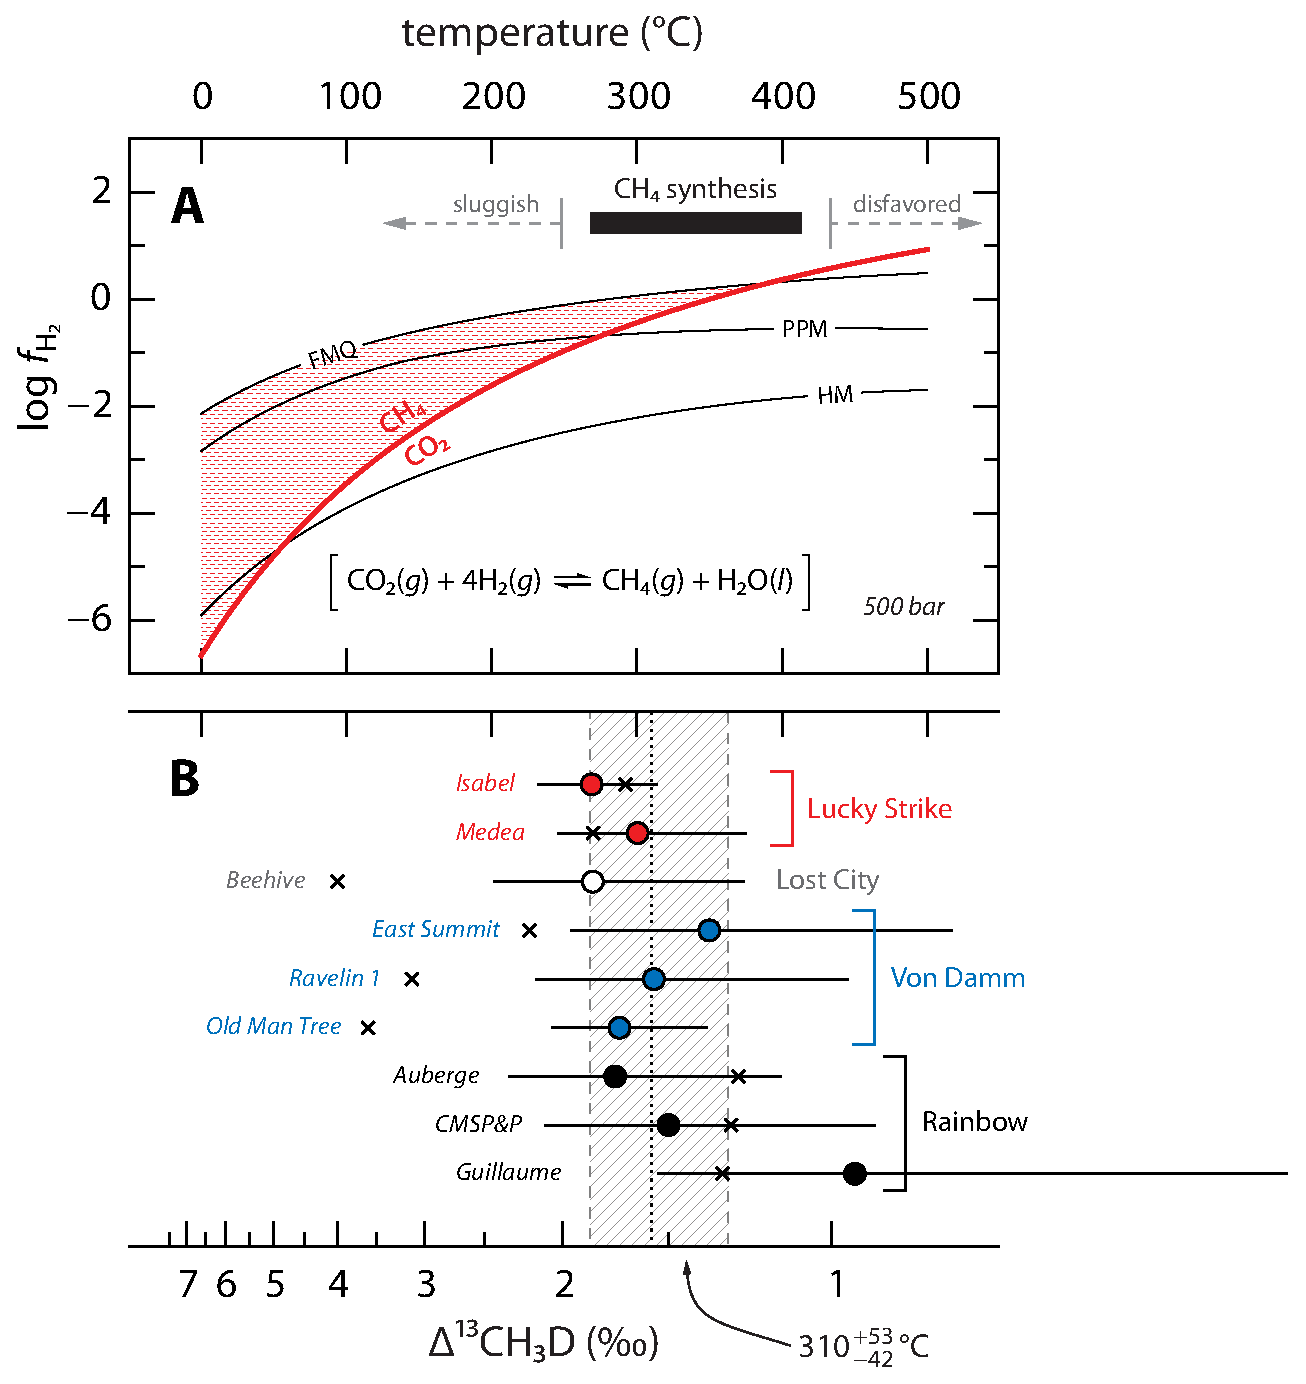
\includegraphics[width=0.75\linewidth]{figures/Fig3.2}
	\caption[Constraints on methane formation and stability from thermodynamics and
	clumped isotopologues]{%
		Constraints on methane formation and stability from thermodynamics and
		clumped isotopologue data. (\textbf{A}) Plot of fugacity of
		H\textsubscript{2} as a function of temperature at 500 bar, after \textcite{Shock_1992}. Red line represents the fugacity of H\textsubscript{2} at
		equilibrium, according to the reaction $ \ce{CO2\text{(\emph{g})}} + 4\ce{H2\text{(\emph{g})}} \leftrightharpoons
\ce{CH4\text{(\emph{g})}} + 2\ce{H2O\text{(\emph{l})}} $, when the fugacities of
		CH\textsubscript{4} and CO\textsubscript{2} are equal, and assuming unit
		activity for H\textsubscript{2}O(\emph{l}). Grey lines represent
		equilibrium H\textsubscript{2} fugacities buffered by the mineral
		assemblages fayalite-magnetite-quartz (FMQ), pyrite-pyrrhotite-magnetite
		(PPM), and hematite-magnetite (HM). Red shaded area represents the
		intersection of regions corresponding to geologically-relevant
		H\textsubscript{2} fugacity and where CH\textsubscript{4} is
		thermodynamically stable relative to CO\textsubscript{2}. The black bar
		represents the temperature range in which the evidence explored in this
		study suggests that methane synthesis is both favorable and facile on
		timescales of relevance to hydrothermal systems. (\textbf{B}) A
		``Caltech plot'' of the clumped isotopologue temperatures of methane
		from studied vents (data and error bars from \autoref{tab:3:1}). Equivalent
		Δ\textsuperscript{13}CH\textsubscript{3}D values are plotted on the
		bottom axis, and are derived from the calibration of \textcite{Wang++_2015_S}.
		The dotted line and gray hatching represent the mean ± 1\emph{s} of the
		Δ\textsuperscript{13}CH\textsubscript{3}D values across all studied
		vents (+1.57 ± 0.28‰, \emph{n} = 9). The × symbols mark measured vent
		temperatures (\autoref{tab:3:2}).
	}
	\label{fig:3:2}
\end{figure*}
